\documentclass[hidelinks, 12pt, oneside]{article}
\usepackage{bookmark}
\usepackage{graphicx}
\usepackage{hyperref}
\graphicspath{{images/}}
\usepackage[utf8]{inputenc}
\usepackage[english]{babel}

\begin{document}
 
%titlepage
\thispagestyle{empty}
\begin{center}
\begin{minipage}{0.75\linewidth}
    \centering
    
%University logo
    
\includegraphics{UPlogo}
    \rule{0\linewidth}{0.15\linewidth}\par

%Thesis title
    {\uppercase{\Large COS 301 Mini Project\par}}
   	{\Large Top Level Integration Testing \par} 
    \vspace{1cm}
%Author's name
    {\normalsize Elana Kuun u12029522\par}
    {\normalsize Hlavutelo Maluleke u12318109\par}
    {\normalsize Estian Rosslee u12223426\par}
    {\normalsize David Breetzke u12056503\par}
    {\normalsize Sylvester Mpungane u11241617\par}
    {\normalsize Phethile Mkhabela u12097561\par}
    {\normalsize Renaldo van Dyk  u12204359\par}
    {\normalsize Antonia Michael  u13014171\par}
    {\normalsize Herman Keuris  u13037618\par}
    {\normalsize Jaco-Louis Kruger  u13025105\par}
    \vspace{1cm}
    
    \href{https://github.com/Jaco-Louis/Top-level-testing.git}{Github Repository}\par
    \vspace{1cm}
%Date
    {\Large April 2015}
\end{minipage}
\end{center}
\clearpage

\tableofcontents

\newpage

\section{Introduction}
This document contains the findings of the various activities performed as per testing of the Buzz Space system top level integration.

\section{Testing Results}
\subsection{Top Level A Testing Results}
\subsubsection{Functional Testing}
\subsubsection{Non-functional Testing} 

\begin{enumerate}
\item Usability:

The system is usable because firstly the necessary actions that a user can take appear in a navigation bar at the top of the screen. Thus it is easy for a novice user to be able to know what to click on and navigate the website. 

The interface is not cluttered, and only basic functionality is displayed on the home screen, making the system more learnable. The buttons are labelled with text rather than with graphical icons, and the text on the button is quite explanatory, which makes their purpose more clear. 

Larger headings are used to label the different sections, for example under the Manage Constraints tab there are large headings to indicate the Existing constraints section and the Add new constraint section. This again contributes to ease of use for the novice furst year user.

Through these mechanisms the system is memborable hence it is also be understandable.  

\item Integratibility:

The system is able to address future integration requirements by providing access to its services using widely adopted public standards such as firstly having seperate npm packages for all the different modules. The packages are stored on Synopia. Also, electrolyte is being used in the server to provide a dependancy injection. The HandleBars server is the main server that needs to be used to test and integrate all the modules on. The routes/index.js, routes/infrastructure.js and routes/content.js files use express to route the different hbs files for the different modules in order to integrate the infrastructure and content subsystems into the main system. 

A seperate file is used to establish the connection to the database to avoid having this done in all the seperate files. Also, global variables are now used such as the global password and username for example. 

A document has been provided via email and a README file has been provided to specify important standards and regulations that must be followed.

The functional code in the seperate packages must be placed in an exportable function taking parameters such as the database or settings, and this is done as part of the electrolyte dependancy injection. 

Exports are also used in the different files to make the code accessible to the other files.

\item Deployability:

The system is deployable on Linux servers as we have run it using Ubuntu 14.04 Linux and the system was able to run. The following screenshot shows the system running on a Linux server:

The system is deployable on an environment using different databases for persistence of the Buzz datatabase because the Handlebars server contains a folder called node\_modules, and it contains the buzz\_database package. This package can easily be swopped out andan alternative database package can be plugged in, that the system can use due to the flexibility of this server. As long as the new package has the same name so that the files that require the database do not need to be changed, no major changes will need to be made.  
//screenshot

The system is deployable in environments where the user authentication credentials and roles are sourced from different repositories. The following screenshot indicates that the Handlebars server contains a folder called node\_modules, and it contains the buzz\_csds package. 
//screenshot

This package can easily be swopped out and an alternative data source package with different credentials and roles can be used, due to the pluggability of the system and dependancy injection employed by the top level team. The new package must just be named the same as the old one to avoid errors where the file is required from the package in the code. 

\end{enumerate}


\subsection{Top Level B Testing Results}

\subsubsection{Functional Testing}

\subsubsection{Non-functional Testing} 

\begin{enumerate}
\newpage
\item Auditability:

\textbf{Description}

The system needs to log all requests and all responses for all user services provided
by the system.

\textbf{Test Results}

The figure below shows that the Buzz Space system is partially auditable, only the requests for the user serves of the system are logged. The logged request only contains:
\begin{itemize}
\item User serves requested.
\item Request object stringified as JSON
\end{itemize}

There are no log responses that are provided by the system, and the serves required to extract information from the audit logs is also not available not provided.

\begin{figure}[h]
  \centering
    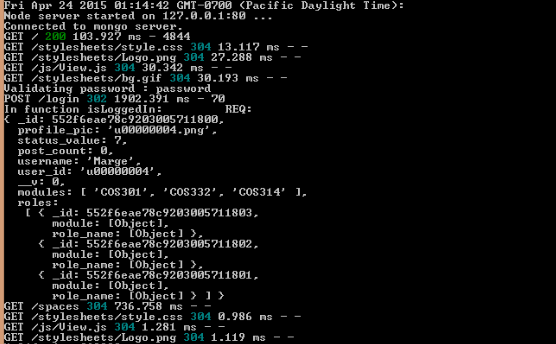
\includegraphics[width=0.85\textwidth]{BuzzBAuditability}
    \caption{Buzz Space B Auditability Test}
\end{figure}

\newpage
\item Testability:

\textbf{Description}

A system needs testabl through:
\begin{itemize}
\item Unit testing components in isolation
\item Integration tests where the components are integrated to the actual environment
\end{itemize}

\textbf{Test Results}
   
The Buzz system is divided into manageable components (modules) for each use case. Breaking the system into these components makes make the system testable through unit testing using mock objects. The Buzz system is a modular system, the system components are pluggable and makes automated integration testing simple as the component is integrated in the entire system.    
\end{enumerate}


\end{document}
